\documentclass[conference]{IEEEtran}
\IEEEoverridecommandlockouts
% The preceding line is only needed to identify funding in the first footnote. If that is unneeded, please comment it out.
\usepackage{cite}
\usepackage{amsmath,amssymb,amsfonts}
\usepackage{algorithmic}
\usepackage{graphicx} % Keep this for figures
\usepackage{textcomp}
\usepackage{xcolor}
\usepackage[hyphens]{url} % Added for better URL handling in bib

\def\BibTeX{{\rm B\kern-.05em{\sc i\kern-.025em b}\kern-.08em
    T\kern-.1667em\lower.7ex\hbox{E}\kern-.125emX}}
\begin{document}

\title{Edge-Driven CO2 and Occupancy Prediction \\ with Certificate Generation for Optimized \\ Classroom Ventilation Systems
% {\footnotesize \textsuperscript{*}Note: Sub-titles are not captured in Xplore and
% should not be used}
% \thanks{Identify applicable funding agency here. If none, delete this.}
}

\author{
    \IEEEauthorblockN{
        Chinthalagari Bhavitha\textsuperscript{1\dag}, 
        Sri Harsha Goruganti\textsuperscript{1\dag}, 
        Vangipuram Sree Raghu Vardhan\textsuperscript{1\dag}, 
        Eliganti Ramalakshmi\textsuperscript{1*}
    }
    \IEEEauthorblockA{
        \textsuperscript{1}Department of Information Technology, Chaitanya Bharathi Institute of Technology, Gandipet, Hyderabad, 500075, Telangana, India.\\
        *Corresponding author. E-mail: \url{eramya2@gmail.com};\\
        Contributing authors: \url{bhavithachinthalagari@gmail.com}; \url{harshagoruganti@gmail.com}; \url{vardhanvsr2004@gmail.com};\\
        \dag These authors contributed equally to this work.
    }
}

\maketitle

\begin{abstract}
Optimizing classroom ventilation is crucial for indoor air quality and occupant well-being. This paper presents an edge computing approach using Internet of Things (IoT) sensors and Long Short-Term Memory (LSTM) networks for intelligent ventilation management in educational settings. Low-cost IoT devices with environmental sensors collect and process data locally. A lightweight LSTM model on the edge predicts ventilation quality and occupancy patterns in real-time, enabling prompt adjustments. The system employs a hierarchical architecture with edge devices for local processing, a fog layer for aggregation, and cloud services for data storage and analysis. This edge-driven system demonstrates effective real-time monitoring and analysis of temperature, humidity, carbon dioxide levels, and occupancy, facilitating optimized classroom conditions and generating environmental quality certificates. The integration of edge computing, machine learning, and IoT offers precise environmental quality evaluation for educational institutions.
\end{abstract}

\begin{IEEEkeywords}
Edge Computing, Indoor Air Quality, CO2 Prediction, LSTM, IoT, Occupancy Monitoring, Smart Ventilation, Certificate Generation
\end{IEEEkeywords}

% Input sections
\section{Introduction}
\label{sec:introduction}

Indoor air quality (IAQ) in educational settings significantly impacts student cognitive function, comfort, and overall health, particularly in densely occupied classrooms \cite{Azuma2018}. Traditional ventilation systems often rely on static thresholds or manual controls, proving inefficient and unresponsive to dynamic changes in occupancy and environmental conditions like Carbon Dioxide (CO\textsubscript{2}) levels \cite{McNeill2022}. Such systems struggle to adapt to fluctuating occupancy, varying room sizes, and diverse usage patterns, leading to inconsistent air quality, potential health concerns, and suboptimal energy consumption.

The primary challenge lies in developing an intelligent, responsive ventilation system capable of real-time data acquisition, accurate prediction of environmental changes, and automated control actions. While cloud-based solutions exist, they often suffer from latency issues unsuitable for immediate environmental adjustments \cite{Idrees2021}. Edge computing, coupled with advancements in Internet of Things (IoT) sensors and deep learning models like Long Short-Term Memory (LSTM) networks, offers a promising alternative by enabling localized data processing and predictive control with minimal delay.

This paper proposes an edge-driven system for real-time CO\textsubscript{2} and occupancy prediction to optimize classroom ventilation. Our approach integrates low-cost IoT sensors for environmental data collection (temperature, humidity, CO\textsubscript{2}, occupancy), a lightweight LSTM model deployed on edge devices for predictive analysis, and certificate generation for environmental quality assurance. The system employs a hierarchical architecture, leveraging edge devices for immediate processing and a fog layer for aggregation, alongside cloud integration for long-term data storage and analysis.

The key contributions of this work are:
\begin{itemize}
    \item Development and edge deployment of a lightweight LSTM model for real-time prediction of CO\textsubscript{2} levels and occupancy patterns in classrooms.
    \item Design and implementation of a hierarchical edge-fog-cloud architecture for efficient data processing, low-latency control, and scalability.
    \item Real-time generation of environmental quality certificates based on continuous monitoring and prediction.
    \item Demonstration of the system's effectiveness in maintaining optimal classroom conditions through adaptive ventilation adjustments.
\end{itemize}

The remainder of this paper is organized as follows: Section \ref{sec:related_work} reviews related work in smart ventilation and edge computing. Section \ref{sec:methodology} details the proposed system architecture and methodology. Section \ref{sec:results} presents the experimental results and evaluation. Finally, Section \ref{sec:conclusion} concludes the paper and discusses future work. 
\section{Related Work}
\label{sec:related_work}

Research in smart ventilation and indoor air quality (IAQ) management has evolved significantly with the integration of Internet of Things (IoT) technologies and machine learning. Early systems often employed rule-based control triggered by simple sensor thresholds, which proved inadequate for dynamic environments. Recent efforts have focused on leveraging IoT sensor networks for real-time data collection and more sophisticated control strategies.

Several studies have explored IoT-based monitoring of various IAQ parameters, including CO\textsubscript{2}, temperature, humidity, and particulate matter (PM). Luo et al. \cite{Luo2021} investigated natural ventilation potential using real-time sensor data, highlighting the gap between potential and actual usage due to occupant behavior. Rastogi et al. \cite{Rastogi2021} developed a context-aware system using k-NN to detect poor ventilation based on multiple pollutants. Others, like Mahbub et al. \cite{Mahbub2021}, integrated IAQ monitoring with other building functions like lighting and fire safety within a single embedded system.

The application of machine learning, particularly deep learning models like Long Short-Term Memory (LSTM) networks, has shown promise for predicting IAQ trends. Tagliabue et al. \cite{Tagliabue2021} used Artificial Neural Networks (ANNs) and Markov models to forecast comfort conditions in educational settings based on CO\textsubscript{2}, temperature, and humidity. Wang et al. \cite{Wang2021} developed a Convolutional Transformer LSTM (CT-LSTM) model for predicting Air Quality Index (AQI), demonstrating superior performance over traditional models. Yang et al. \cite{Yang2021} proposed a hybrid Bayesian Optimization-Empirical Mode Decomposition-LSTM (BO-EMD-LSTM) method for highly accurate long-term CO\textsubscript{2} prediction. These predictive capabilities enable proactive ventilation control rather than reactive adjustments.

The trend towards edge computing is prominent in recent IAQ research, aiming to reduce latency, enhance privacy, and improve responsiveness compared to purely cloud-based architectures. Idrees et al. \cite{Idrees2021} proposed an edge architecture for real-time monitoring using low-cost sensors and local processing. Taştan and Göközan \cite{Tastan2019} developed an IoT e-nose using edge computing for rapid anomaly detection. Zhang et al. \cite{Zhang2021} deployed an LSTM model directly on an ESP32 for CO\textsubscript{2} forecasting, enabling proactive control and energy savings. Similarly, Sun et al. \cite{Sun2022} implemented model predictive control (MPC) on a Raspberry Pi for real-time optimization of CO\textsubscript{2} and energy use.

While existing research has explored IoT-based monitoring, predictive modeling, and edge deployment individually or in partial combinations, our work integrates these aspects into a cohesive system specifically targeting classroom environments. We combine real-time, multi-sensor data acquisition (including occupancy) with a lightweight LSTM model deployed at the edge for simultaneous CO\textsubscript{2} and occupancy prediction, coupled with automated environmental quality certificate generation. This holistic edge-driven approach aims to provide a responsive, scalable, and verifiable solution for optimizing ventilation in educational spaces, addressing the limitations of previous systems in terms of combined prediction, real-time edge control, and quality assurance. 
\section{System Design and Methodology}
\label{sec:methodology}

Our proposed system employs a hierarchical Edge-Fog-Cloud architecture (illustrated in Figure~\ref{fig:system_architecture}) designed for real-time monitoring, prediction, and control of classroom environmental conditions, primarily focusing on CO\textsubscript{2} levels and occupancy.

\begin{figure}[htbp] % Use [htbp] for positioning suggestion
    \centering
    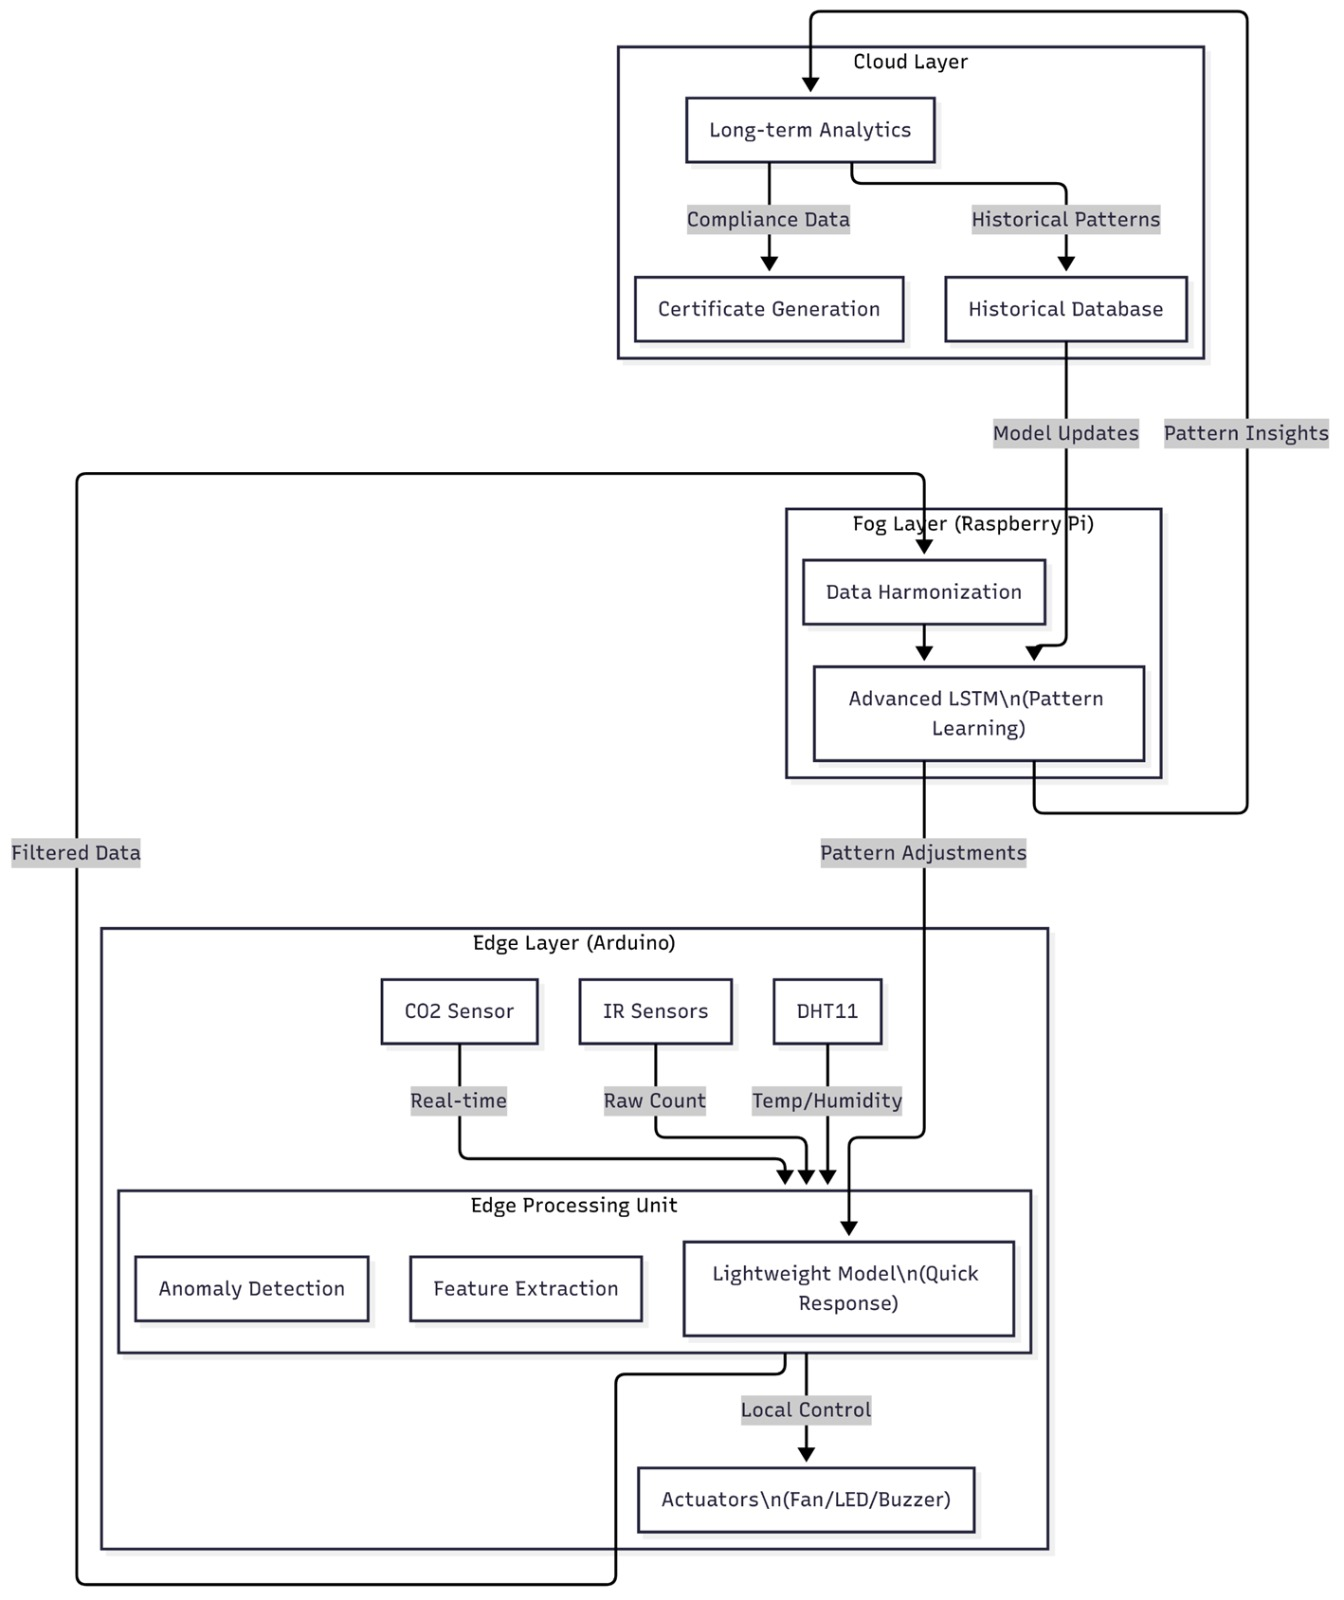
\includegraphics[width=0.9\linewidth]{figures/workflow.jpg (1).jpeg} % Use linewidth for responsiveness
    \caption{Proposed System Flow Architecture (Edge-Fog-Cloud).}
    \label{fig:system_architecture}
\end{figure}

\subsection{System Architecture}

\textbf{Edge Layer:} Consists of Arduino Uno based nodes deployed in each monitored classroom. Each node is equipped with:
\begin{itemize}
    \item An MQ135 sensor for CO\textsubscript{2} concentration measurement (400-2000 ppm range).
    \item A DHT11 sensor for temperature and humidity readings.
    \item Paired Infrared (IR) sensors at doorways for bidirectional occupancy counting.
    \item A 16x2 LCD for displaying real-time status (temperature, humidity, air quality).
    \item Actuators: 12V DC fans (controlled via relay modules), LEDs (status indicators), and buzzers (alerts).
\end{itemize}
The Arduino units perform initial data acquisition, basic filtering, local actuation (immediate response to critical thresholds), and transmit processed sensor readings to the Fog layer via serial communication (USB, 9600 baud).

\textbf{Fog Layer:} A Raspberry Pi 4 (4GB RAM) acts as the central fog controller. Its responsibilities include:
\begin{itemize}
    \item Aggregating data streams from multiple Edge nodes.
    \item Executing the pre-trained LSTM model for CO\textsubscript{2} and occupancy prediction.
    \item Implementing decision logic based on predictions and custom metrics (KPIv, Room Quality Score).
    \item Sending control commands back to Edge nodes (e.g., activate fans).
    \item Communicating with the Cloud layer for data logging and synchronization.
\end{itemize}
Python is used for programming the Fog layer, utilizing libraries like TensorFlow/TensorFlow Lite, NumPy, Pandas, and Scikit-learn.

\textbf{Cloud Layer:} ThingSpeak is utilized for cloud functionalities:
\begin{itemize}
    \item Long-term storage of historical sensor data and predictions.
    \item Data visualization through dashboards.
    \item Automated generation of environmental quality certificates based on aggregated performance data.
    \item Potential for remote monitoring and triggering model updates.
\end{itemize}

\subsection{Data Collection and Preprocessing}

Real-time data (CO\textsubscript{2}, temperature, humidity, occupancy count) is collected every few minutes (configurable, typically 3-5 mins) by the Edge nodes. Before model training (offline) and prediction (online on Fog), the data undergoes preprocessing:
\begin{itemize}
    \item Handling Missing Values: Time-based interpolation is used for offline dataset preparation.
    \item Normalization: Min-Max scaling is applied to features to ensure values are within a consistent range (e.g., 0 to 1), preventing features with larger magnitudes from dominating the learning process.
    \item Sequencing: Data is structured into sequences using a sliding window approach (e.g., using the last 10-15 timesteps) to provide temporal context for the LSTM model.
    \item Train/Validation/Test Split: For offline training, the dataset is split chronologically (e.g., 70%/20%/10%) to maintain temporal integrity.
\end{itemize}

\subsection{LSTM Predictive Model}

A Long Short-Term Memory (LSTM) network is employed for its ability to capture long-range temporal dependencies in time-series data.

\textbf{Architecture:} The model consists of:
\begin{itemize}
    \item An input layer accepting sequences of features (CO\textsubscript{2}, temperature, humidity, occupancy).
    \item Two stacked LSTM layers (64 units followed by 32 units) to learn hierarchical temporal patterns.
    \item Dropout layers between LSTM layers to mitigate overfitting.
    \item A Dense output layer producing the predicted CO\textsubscript{2} concentration for the next timestep.
\end{itemize}

\textbf{Training:} The model was trained offline using the preprocessed dataset.
\begin{itemize}
    \item Loss Function: Mean Squared Error (MSE) was used to minimize the difference between predicted and actual values.
    \begin{equation}
    \mathcal{L}_{\text{MSE}} = \frac{1}{N} \sum_{i=1}^{N} (y_i - \hat{y}_i)^2
    \label{eq:mse_methodology}
    \end{equation}
    \item Optimizer: Adam optimizer was used for efficient gradient descent.
    \item Epochs: Trained for up to 200 epochs with EarlyStopping based on validation loss to prevent overfitting.
    \item Learning Rate Scheduling: Adaptively adjusted the learning rate during training.
\end{itemize}
The trained model weights and scaler were saved (`pretrained_lstm.weights.h5`, `pretrained_scaler.joblib`) and converted to TensorFlow Lite format for efficient deployment on the Raspberry Pi (Fog layer).

\subsection{Prediction Logic and Control}

The Fog layer uses the deployed LSTM model to predict future CO\textsubscript{2} levels. Based on these predictions and current sensor readings, it calculates two key metrics:

\textbf{KPIv (Key Performance Indicator for Ventilation):} Quantifies ventilation quality based on CO\textsubscript{2} and occupancy.
\begin{equation}
KPIv = 
\begin{cases} 
2.0 & \text{if } CO_2 > 1000 \, \text{ppm} \\
\frac{CO_2 - 400}{20 \times actual\_people} & \text{if } actual\_people > 0 \\
0.5 & \text{if } est\_people > 0, actual\_people = 0 \\
0.0 & \text{otherwise}
\end{cases}
\label{eq:KPIv_methodology}
\end{equation}
where actual\_people is the count from IR sensors, and est\_people represents estimated occupancy.

\textbf{Room Quality Score:} Provides a holistic score incorporating multiple factors.
\begin{multline} 
    Score = 5 \times KPIv + 0.2 \times |Temp - 24| \\
    + 0.3 \times \frac{CO_2}{1000} + 0.1 \times Occupancy
    \label{eq:Score_methodology}
\end{multline}
This score helps compare classrooms and trigger broader actions.

Based on these metrics and predictions, the Fog layer sends commands to the Edge nodes to activate fans for ventilation, display status updates on LCDs, and trigger alerts (LEDs, buzzers) if thresholds are breached or predicted to be breached. 
\section{Results and Evaluation}
\label{sec:results}

This section presents the results obtained from the implementation and deployment of the proposed edge-driven classroom environmental monitoring and ventilation optimization system.

\subsection{Experimental Setup}
The system was deployed across two classrooms, utilizing the hardware architecture described in Section \ref{sec:methodology} (Arduino nodes, Raspberry Pi fog controller, sensors), shown in Figure~\ref{fig:hardware_photo}. Environmental data (Temperature, Humidity, CO\textsubscript{2}, Occupancy) was collected continuously over a monitoring period (e.g., several days, as indicated by ThingSpeak data from April 13-19 in the thesis). Data was logged locally and synchronized with the ThingSpeak cloud platform at regular intervals (approx. 5-15 minutes, based on descriptions).

\begin{figure}[t]
  \centering
  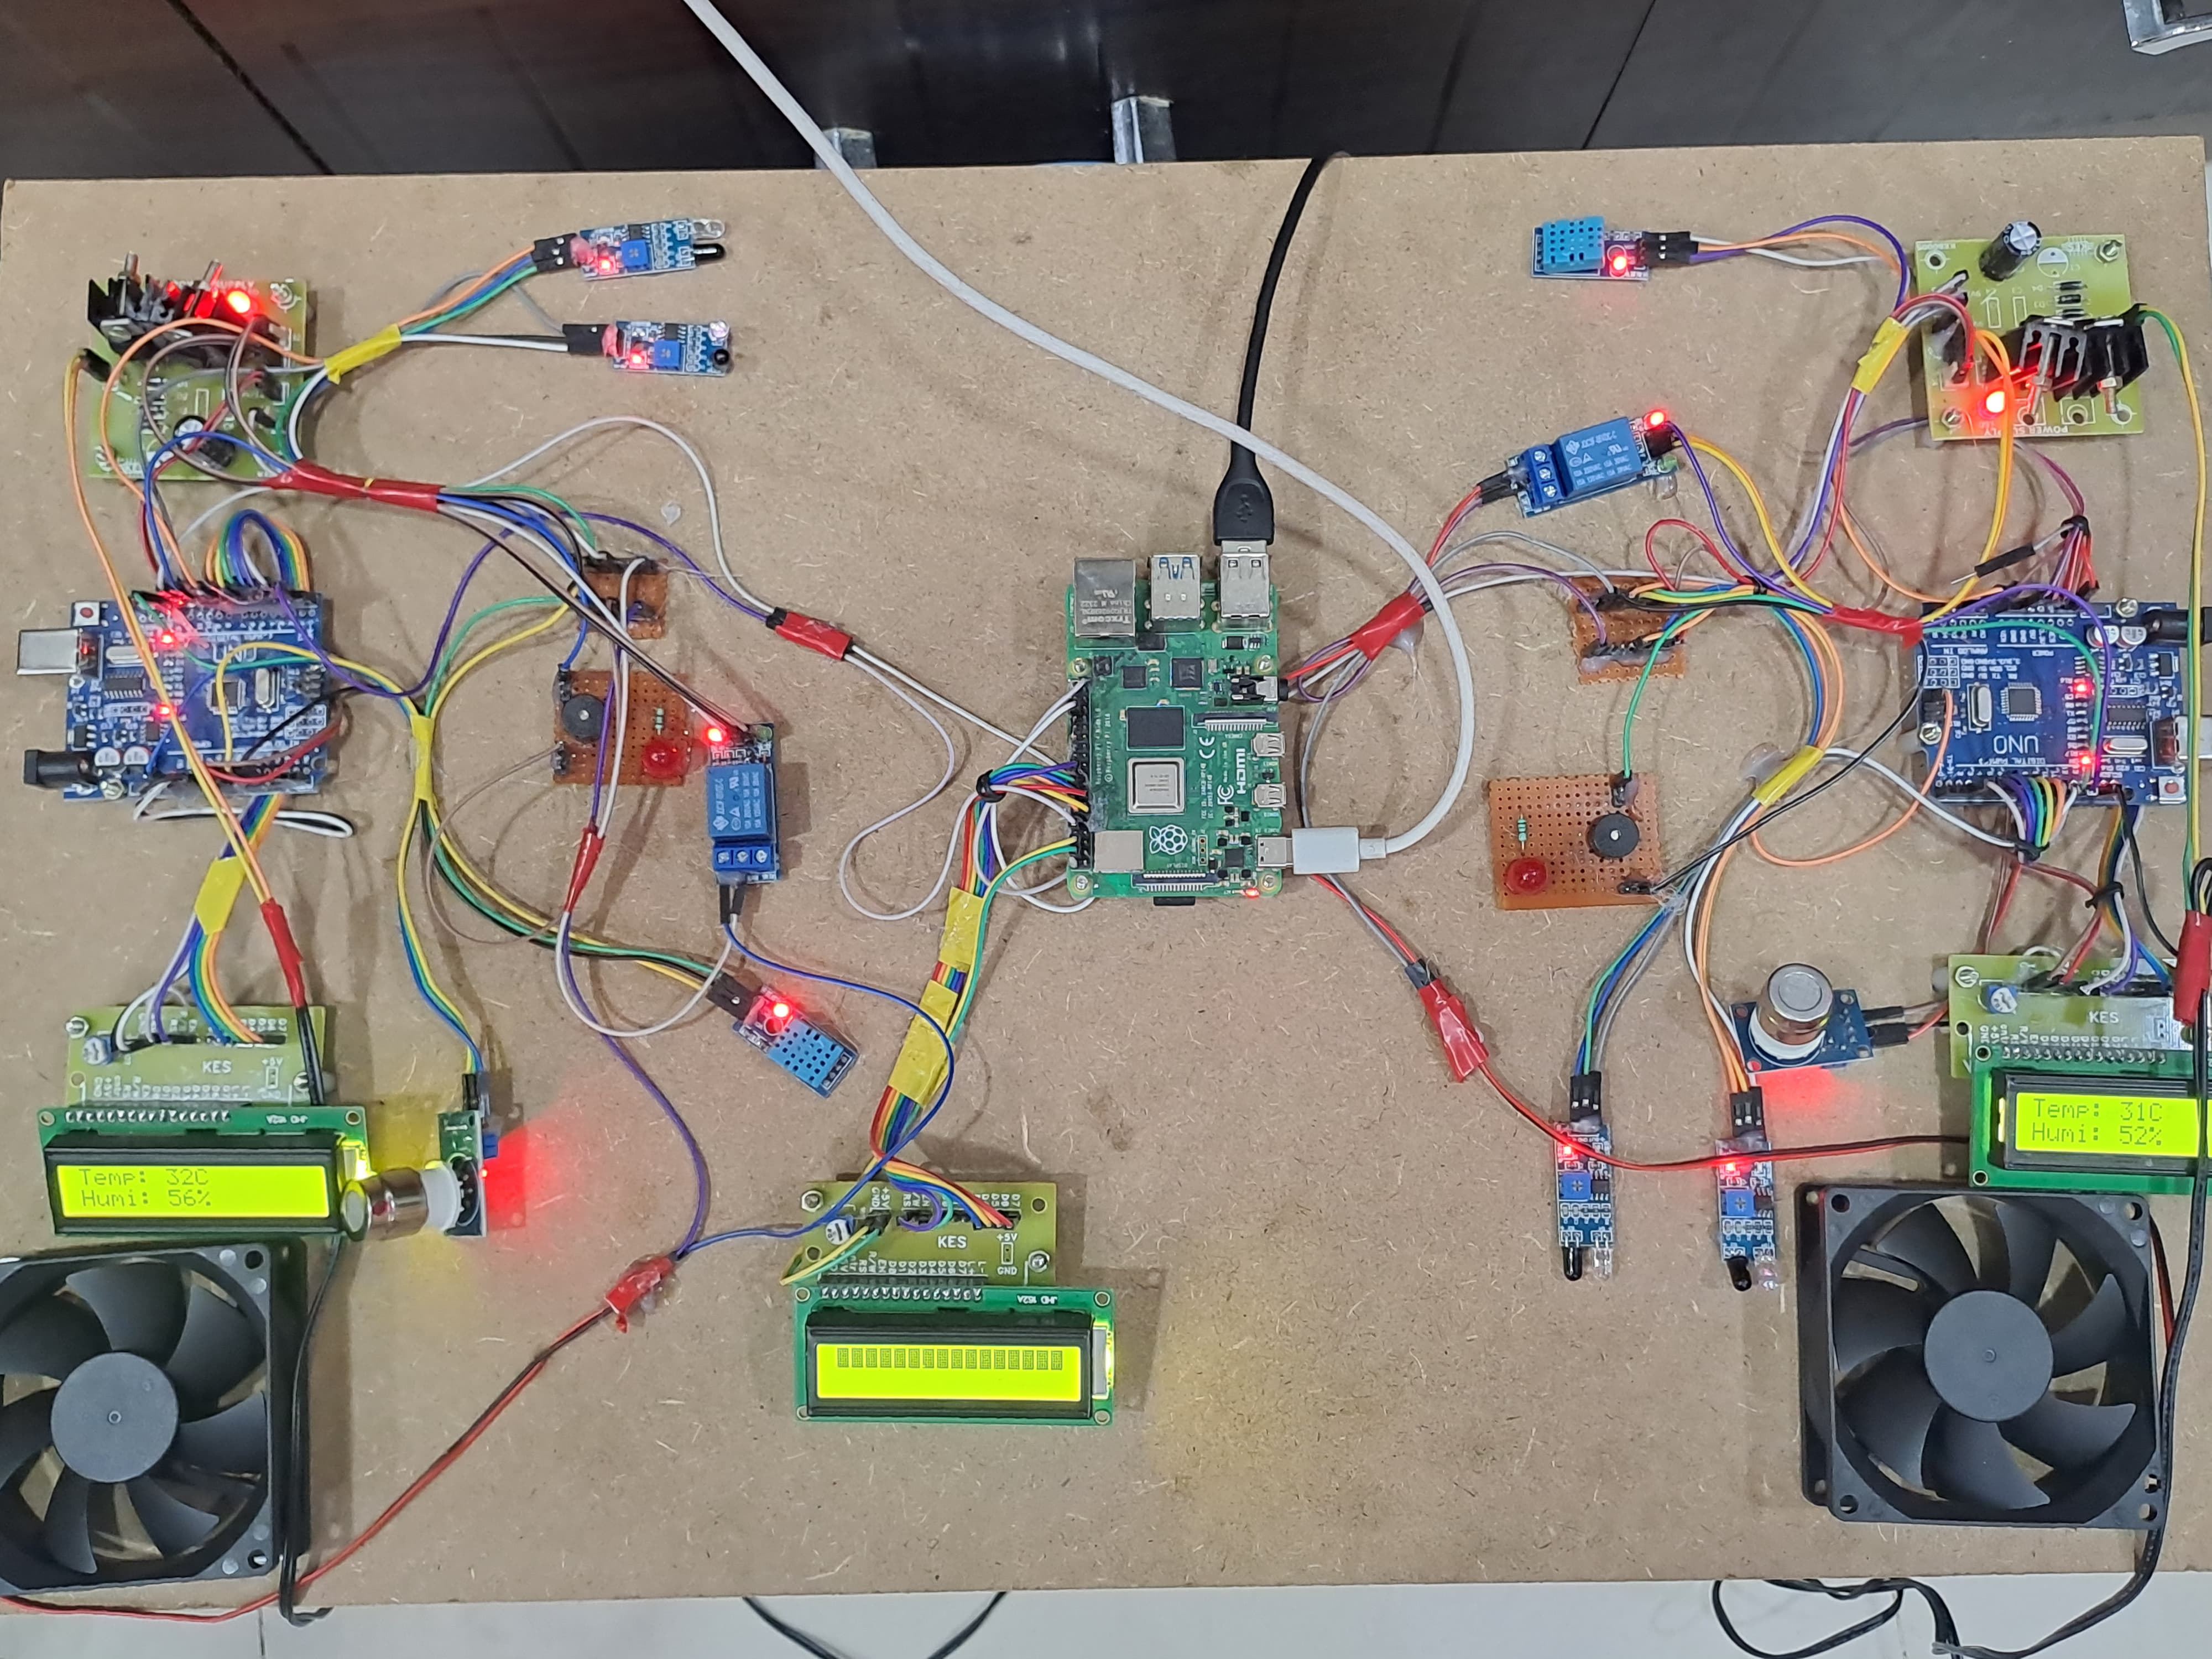
\includegraphics[width=\columnwidth]{figures/kit.jpg.jpeg} % Changed width
  \caption{Hardware Implementation of the Edge-Based IoT System.}
  \label{fig:hardware_photo}
\end{figure}

\subsection{Data Collection and System Operation}
Real-time sensor data was successfully collected and processed by the Edge and Fog layers. ThingSpeak visualizations (Figures~\ref{fig:thingspeak_cls1} and \ref{fig:thingspeak_cls2}) confirmed consistent data logging. During the monitored period, observed environmental parameters included:
\begin{itemize}
    \item Temperature: Fluctuating generally between 31.0°C and 32.0°C.
    \item Humidity: Varying between 36.0\% and 40.0\%.
    \item CO\textsubscript{2}: Concentrations typically observed between 11-13 ppm in the provided sample, but showing potential spikes correlating with occupancy or ventilation changes (as suggested by the description of graphs in the thesis).
    \item Occupancy: Variable rates observed, reflecting classroom usage patterns.
\end{itemize}
The system demonstrated its ability to process this data in real-time, calculate the KPIv and Room Quality Score, and provide actionable recommendations. Log outputs and LCD displays (Figure~\ref{fig:lcd_output}) confirmed the system's capability to compare classroom conditions and suggest the optimal room based on calculated scores (e.g., recommending Classroom 1 with a score of 61.35 over Classroom 2 with 114.74 in one instance).

\begin{figure}[t]
  \centering
  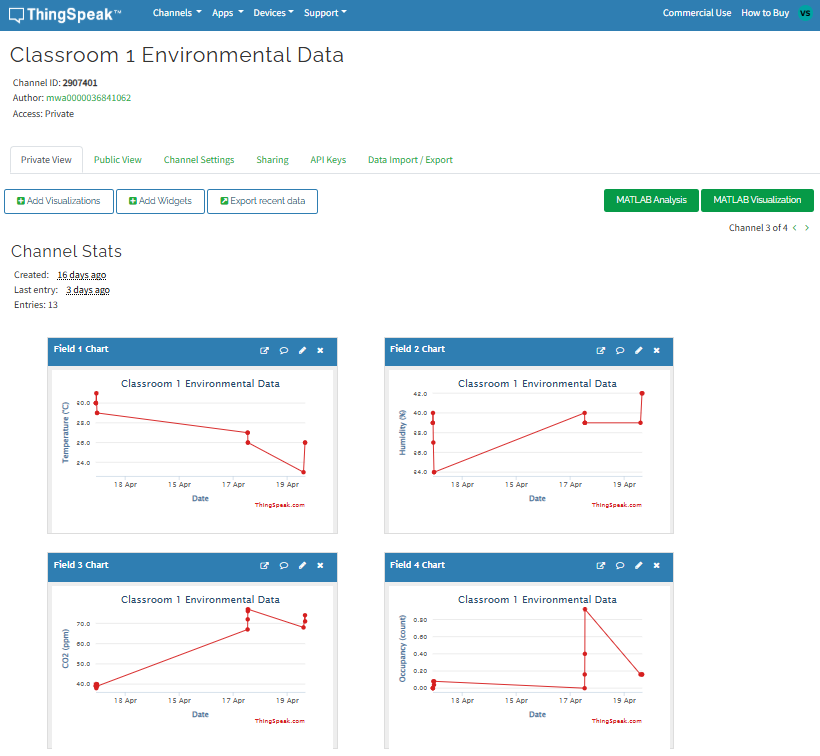
\includegraphics[width=\columnwidth]{figures/cls1.png} % Changed width
  \caption{ThingSpeak Data Visualization for Classroom 1.}
  \label{fig:thingspeak_cls1}
\end{figure}

\begin{figure}[t]
  \centering
  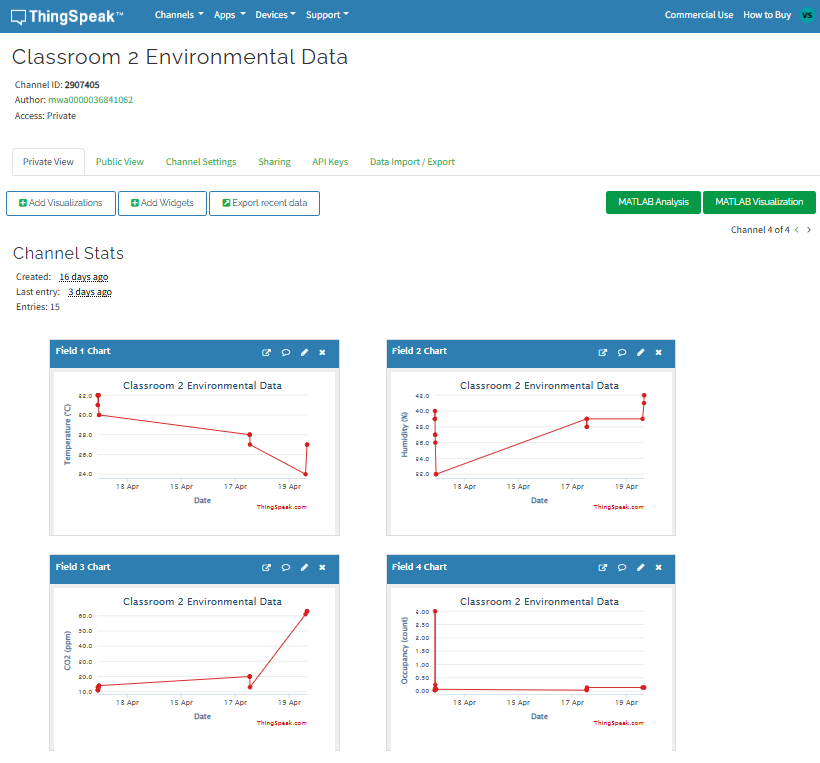
\includegraphics[width=\columnwidth]{figures/cls2.png} % Changed width
  \caption{ThingSpeak Data Visualization for Classroom 2.}
  \label{fig:thingspeak_cls2}
\end{figure}

\begin{figure}[t]
  \centering
  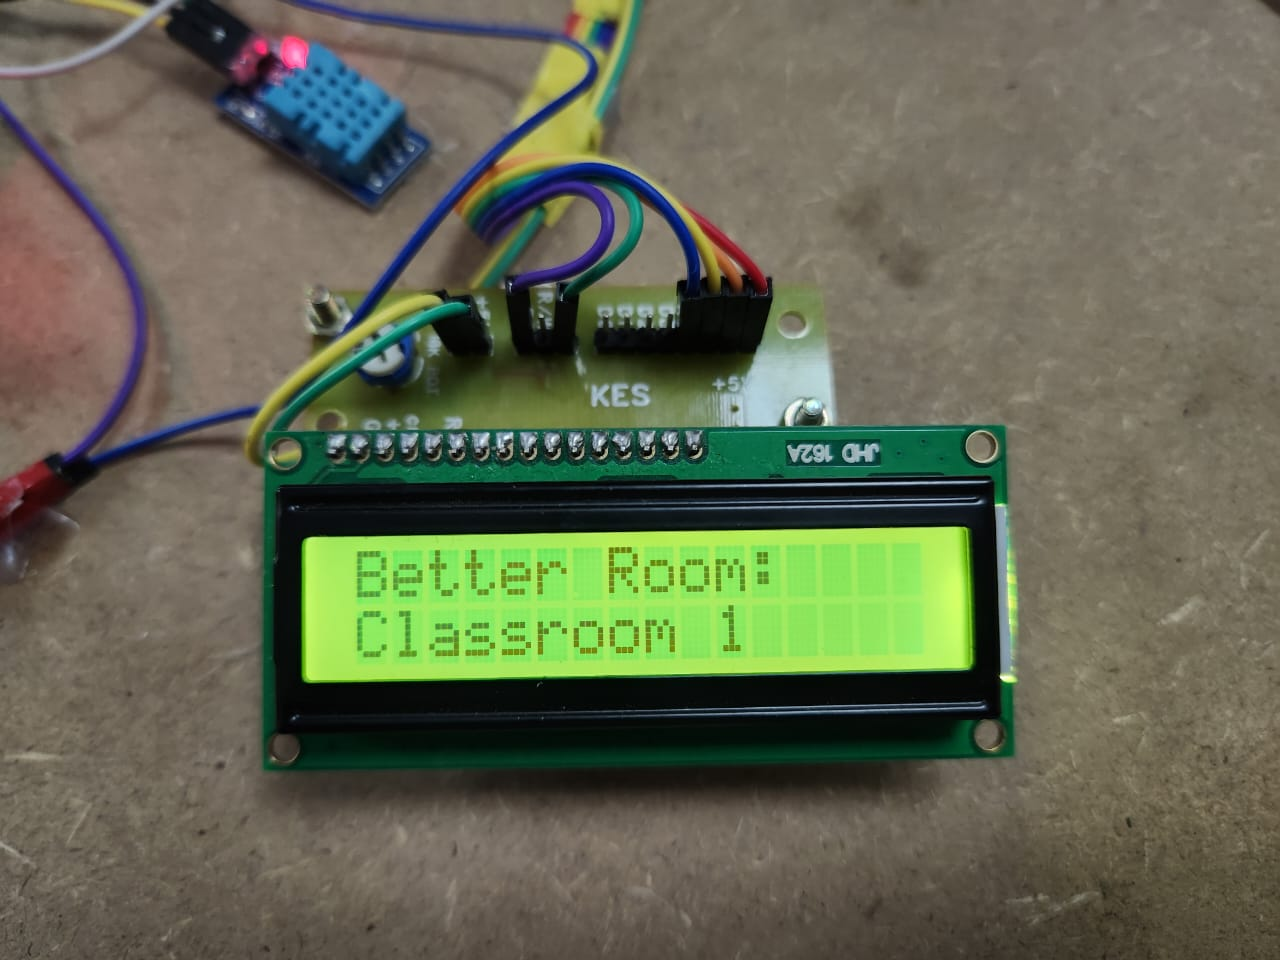
\includegraphics[width=0.8\columnwidth]{figures/lcd.jpeg} % Changed width
  \caption{LCD Output Display Indicating Recommendation of Optimal Classroom.}
  \label{fig:lcd_output}
\end{figure}

\subsection{LSTM Model Performance}
The LSTM model was trained offline on a harmonized dataset derived from multiple sources, preprocessed using forward-fill for missing values and Min-Max scaling, and structured into sequences of 10 timesteps. The training utilized the Adam optimizer and Mean Squared Error (MSE) loss, running for 5 epochs with early stopping and learning rate adjustment (as detailed in Section \ref{sec:methodology}). The pre-trained model, evaluated on the test set, achieved a final loss (MSE) of 0.0012 and a Mean Absolute Error (MAE) of 0.0143. This level of performance indicates the model's capability to predict environmental trends with reasonable accuracy. The trained model, deployed on the Fog layer (Raspberry Pi), successfully processed real-time sensor sequences to generate predictions. The system's ability to utilize these predictions alongside current data for calculating KPIv and Room Quality Score confirms the practical integration of the ML model into the control loop.

\subsection{Certificate Generation}
The automated certificate generation component successfully processed the collected environmental data stored via ThingSpeak. A sample generated certificate (Figure~\ref{fig:certificate_example}) demonstrated the system's ability to:
\begin{itemize}
    \item Aggregate data over a specified period (e.g., 6 readings shown).
    \item Calculate average, minimum, and maximum values for key parameters (Temp, Humidity, CO\textsubscript{2}, Occupancy).
    \item Compute the KPIv based on the collected data.
    \item Assign an overall environmental quality grade (e.g., A+ with a score of 95/100 achieved in the sample).
\end{itemize}
This validates the end-to-end functionality of the system, from data collection and analysis to formal quality reporting.

\begin{figure}[t]
  \centering
  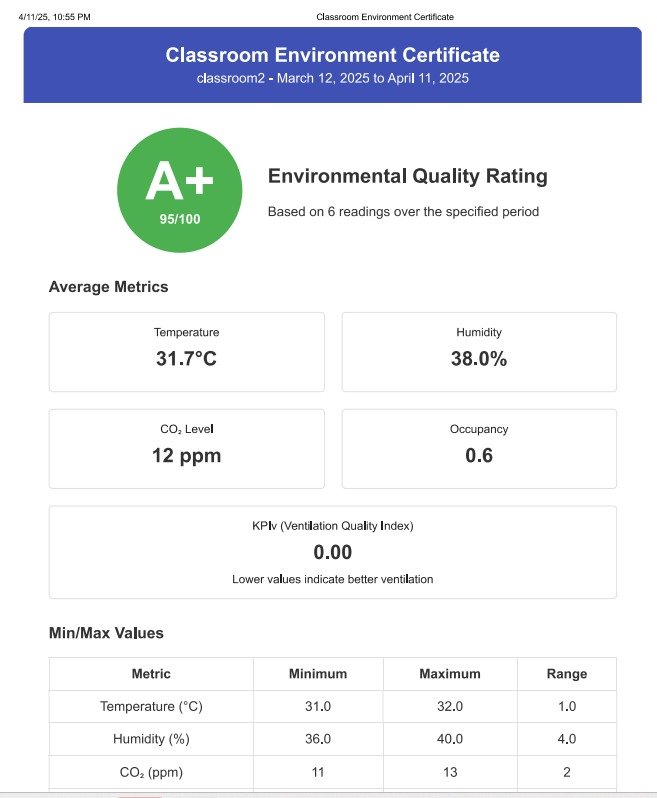
\includegraphics[width=\columnwidth]{figures/image (4).png} % Changed width
  \caption{Example Generated Classroom Environmental Quality Certificate.}
  \label{fig:certificate_example}
\end{figure}

Overall, the results demonstrate the feasibility and effectiveness of the proposed edge-driven system in monitoring classroom environments, utilizing LSTM predictions for intelligent assessment, and providing automated control and quality certification. 
\section{Conclusion and Future Work}
\label{sec:conclusion}

This paper presented an edge-driven system for CO\textsubscript{2} and occupancy prediction aimed at optimizing classroom ventilation. By integrating real-time IoT sensor data (CO\textsubscript{2}, temperature, humidity, occupancy) with an LSTM predictive model deployed on a Raspberry Pi (fog layer) controlling Arduino-based edge nodes, the system demonstrated effective environmental monitoring and proactive ventilation management. Key achievements include the successful implementation of the hierarchical edge-fog-cloud architecture, accurate prediction of environmental trends enabling calculations of KPIv and Room Quality Score, and the automated generation of environmental quality certificates via ThingSpeak integration.

The results validate the feasibility of using lightweight LSTM models on edge/fog devices for real-time analysis and control in resource-constrained environments like classrooms. The system effectively bridges low-cost IoT deployment with intelligent building management principles, offering a data-backed approach to ensuring healthier indoor air quality. The ability to provide verifiable environmental quality certificates adds a layer of accountability and transparency.

Future work will focus on enhancing the system's practicality and scalability. Key directions include:
\begin{itemize}
    \item \textbf{Wireless Communication:} Replacing the current wired serial connection between edge and fog layers with wireless protocols like Zigbee or LoRaWAN to improve deployment flexibility.
    \item \textbf{Model Enhancement:} Training the LSTM model on larger, more diverse datasets incorporating data from various room types and conditions to improve generalizability and accuracy.
    \item \textbf{Expanded Sensing:} Incorporating additional sensors for parameters like Particulate Matter (PM2.5) and Volatile Organic Compounds (VOCs) to provide a more comprehensive IAQ assessment.
    \item \textbf{HVAC Integration:} Interfacing the system directly with building HVAC systems for fully automated and optimized ventilation control, moving beyond simple fan actuation.
    \item \textbf{Advanced ML Techniques:} Exploring techniques like federated learning for enhanced privacy and adaptive learning for real-time model fine-tuning directly on edge/fog devices.
    \item \textbf{Scalability Testing:} Deploying the system across a larger number of classrooms or zones to evaluate performance and management at scale.
\end{itemize}
By pursuing these enhancements, the system can evolve into a more robust, scalable, and intelligent solution, contributing significantly to the development of healthier, energy-efficient, and data-driven educational environments. 

% Optional Acknowledgement Section
% \section*{Acknowledgment}
% The authors would like to thank...

% Bibliography
\bibliographystyle{IEEEtran}
\bibliography{bibliography/references}


\end{document} 